\subsection{Application Features}
\subsubsection{Graphic User Interface with PyTorch}
The purpose of this project(PyTorch GUI) is to develop a Python-based GUI(Graphical User Interface) 
which uses PyTorch Libraries and its an open-source deep learning graphic user interface such as Expresso for Caffe, NVidia DIGITS for Theano, Caffe, Torch and Tensorflow.
\par Even though there are many graphical user interfaces which provide numerous tools for deep learning purposes but unfortunately they are not
compatible with PyTorch Library at the moment we began this project. Therefore, we proposed an application that is an graphical user interface for PyTorch and provides the abilities to use all deep learning features provided by the Pytorch framework.
\\\
\par PyTorch GUI provides a complete featured deep learning application with variety of options.
The \textbf{Qt4 Designer} is used for front hand in this project which provides all graphical objects such as Form, Tabs, Buttons, Drop-down-menus, Radio-buttons, Check-boxes etc. 
For the back hand, Python language with PyTorch framework are used to import, create the network, train, and classify the datasets. All features of this application is 
\\\
\newpage
% Data tab  Explanation
The first Tab is \textbf{"Data"} Tab, which is responsible for importing datasets for further operations.
\\\
\textbf{In this Tab we have the following options:} 
\begin{enumerate}
    \item Drop-down list \newline
        Contains different datasets such as CIFAR10, CIFAR100, MNIST. These datasets holds different types of images for training in various image processing systems and Machine learning.
        The user has to select the type data he will import.
    \item Training set \newline
        User may check this option in order to train and classify the data imported.
    \item Testing set \newline
        User may check this option in order to Test whether our Train data is closest to the accurate result or not.
    \item Open data \newline 
        %The user can display in "Data Table" the contains the dataset.
        The user can import data via this button. It will be then displayed in the "Data table" on the left.
    \item Clear data \newline
        Will clear imported data in case if the user want to import another type of data.
    \item Data table \newline
        The imported dataset will be displayed in the following "Data Table". 
\end{enumerate}

\begin{figure}[h!]
    \centering 
    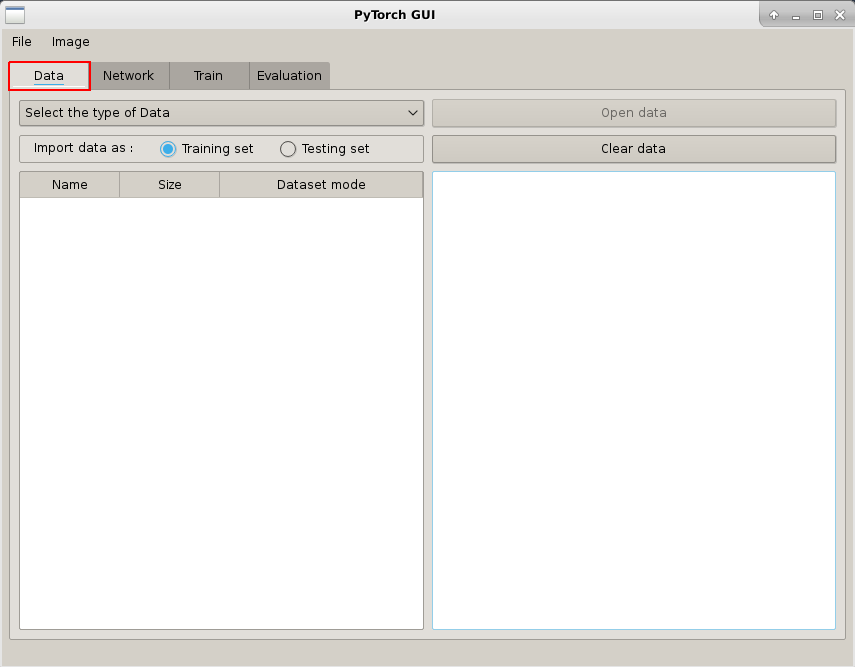
\includegraphics[scale=0.4]{figures/app_screen_shoots/Data_tab.png}
    \caption{Data Tab}
\end{figure}



\newpage
% Network tab Explanation
The Network tab enables the users to choose their desire neuron network according their needs. \newline 
\textbf{There are the following options and objects in this tab:}
\begin{enumerate}
    \item This widget is used to show the graph of the network.
    \item Select a layer \newline
        The first drop-down (from left side) allows the users to select the layer such as Conv1d, Conv2d, Conv3d and so on.
    \item Add a layer \newline
    Once a layer is selected it will display a pop-up where the user can edit the layer's parameters.
    He will then have to clicked on \textbf{add} to add the layer into the current network.
    \item Select an activation layer \newline
        The next down (drop-down list) is used to select activation function for example ReLU, ReLU6, ElU, Tanh and so on.
    \item Add an activation function \newline
    Once an activation function is selected it will display a pop-up where the user can edit the parameters, he will then click on \textbf{Add} to add the function to the current network.
    \item Select a layer\newline
    In this drop-down, the user can select an existing layer of the network.
    \item Edit layer\newline
    Once a layer is selected in the previous drop-down, the user can edit the layer (rename, change parameters, set a nextLayer)
    \item Set as first layer\newline
    Once a layer is selected in the previous drop-down the user can set it as the first layer of the neural network.
    
    \item Select a loss function \newline
        In this drop-down, we choose a loss function.
    \item Confirm \newline
    Once a loss function is selected, it will open a pop-up where user can edit the parameters.
    He will then have to click on \textbf{set} to validate the function.
    \item Select optimizer function \newline
    In this drop-down the user can select an \textbf{Optimizer function} (load from a database in background). 
    \item Confirm \newline
    Once an optimizer function is selected, it will display a pop-up where the user can edit the parameters. 
    He will then have to click on \textbf{Set} to validate the function.
    \item Load \newline
    It opens a file-explorer in which the user can only select json files, if the file is correct it will load the layers that composed a neural network and put them into our current network dictionary layers.
    
    \item Save \newline
    The users can save the current dictionary that contains all the layers that compose the current neural network into a json file, a file explorer will display and the user can choose the Path he want to save his file.
\end{enumerate}

\begin{figure}[h!]
    \centering 
    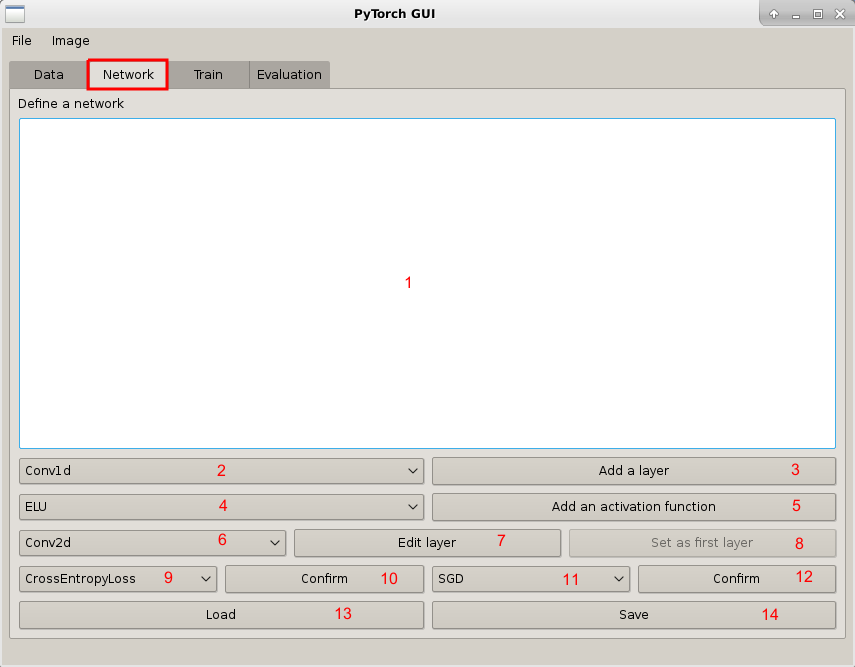
\includegraphics[scale=0.4]{figures/app_screen_shoots/Network_tab.png}
    \caption{Network Tab}
\end{figure}


\newpage
% Train tab Explanation

\\\
\textbf{The Train tab is used to Train and classify the imported datasets There are the following options and objects in this tab:}
\begin{enumerate}
    \item Train set \newline
        In Training set we select the type of dataset that we have already chose such as CIFAR10 or any other type.
    \item Number of epochs \newline
        Number of epochs are the number of iterations that we train the dataset.
    \item Batch size \newline
        The whole dataset will be divided according to the given number to Batch size and each divided group would be processed by a thread.
    \item Worker number \newline
        Divides the process on all of the core exists on the machine where this application might run.
\end{enumerate}

\begin{figure}[h!]
    \centering 
    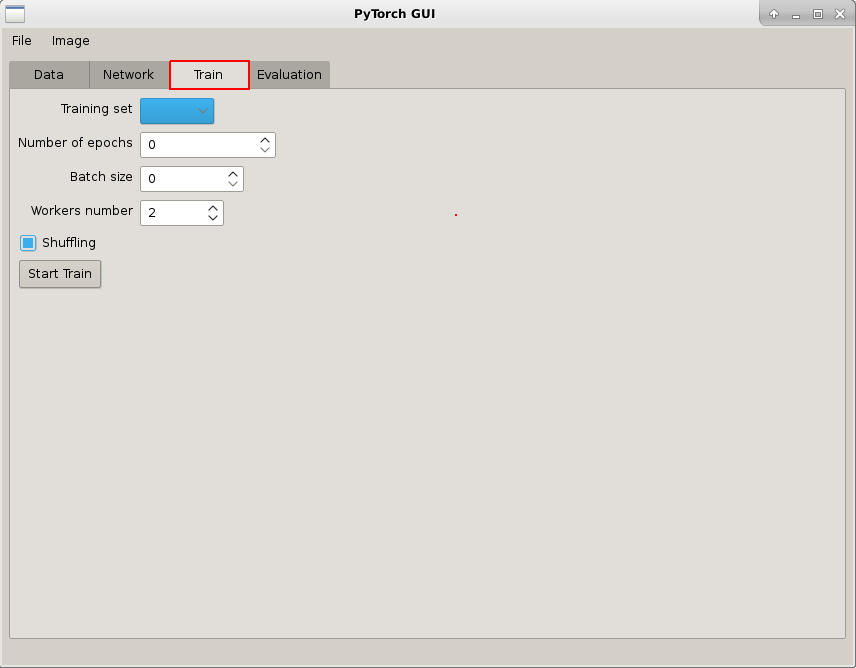
\includegraphics[scale=0.4]{figures/app_screen_shoots/Train_tab.png}
    \caption{Train Tab}
\end{figure}


\textbf{In this tab the end result will be evaluated to check that how far our result is from desired value and we have the following objects:}
This tab for the moment is not working.

\begin{figure}[ht!]
    \centering 
    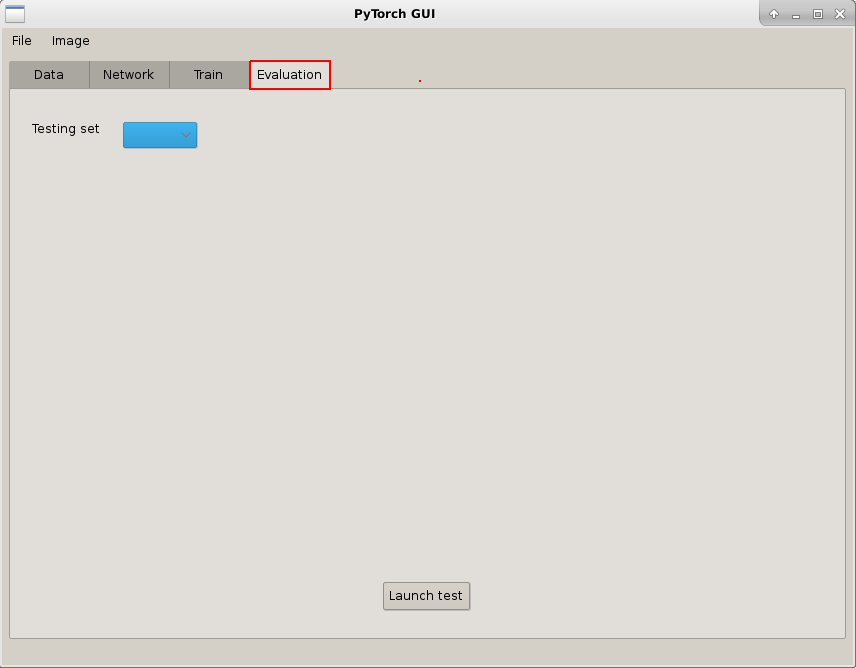
\includegraphics[scale=0.4]{figures/app_screen_shoots/Evaluation_tab.png}
    \caption{Evaluation Tab}
\end{figure}

\newpage
\subsection{Edit neural network from scratch}
Users have two different way for building a Neural Network. Etheir from scratch or from an pre-loaded model.

\begin{figure}[h!]
    \centering 
    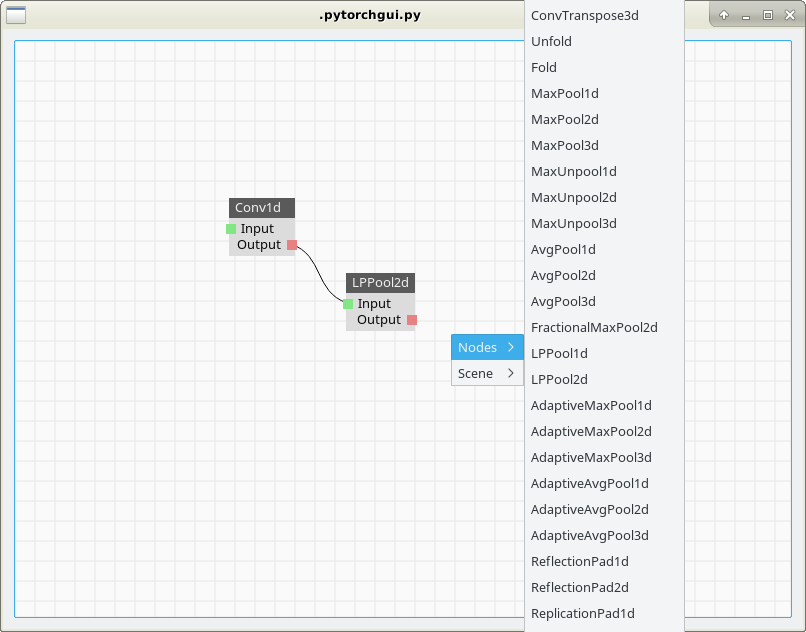
\includegraphics[scale=0.4]{figures/fromscratch.png}
    \caption{From scratch feature}
\end{figure}

From scratch user just have to click on add a layer and he can see the graph representation.

\section{Problems of the application}
\subsection{Non-working features}
Some features are not totally implemented:
\begin{itemize}
    \item Load json from scratch 
    \item Evaluate
    \item Forward function in training, we have to code it
\end{itemize}
\subsection{Non-implemented features}
Some features are almost not implemented, so their functionalities are not currently working
\begin{itemize}
    \item Fetch the layer type set in the json files and pass them to the scratch module
    \item Load a model from the scratch module and show the graph representation
\end{itemize}
\subsubsection{The Evaluation Class}
The evaluation methods are already present in the Evaluation class, but we didn't include them in the rest of the application

\subsubsection{Training result display}
The display of the training is currently printed in the console.
An improvement of this could be to print graphs in the application.
\subsubsection{Exception handling}
There are two types of exceptions that are returned by the application :
\begin{itemize}
    \item our own exceptions, from our application
    \item exceptions from PyTorch
\end{itemize}
For the moment, all the exceptions are printed in the console. To handle them, we could notify the user by displaying a popup in the graphical interface.

\section{Test}
To make sure the application is working properly, we need to test all features with determined data sets.

\textbf{Examples of tests :}
\begin{itemize}
\item Importing a set of data, edit its variables and export it.\newline
To test this functionality we can simply try do import a data supported by Pytorch. We can use the Pytorch tutorials to test the importation of data like Cifar10.
We import as a training set the Cifar10 dataset, it will create a data object of size 50000, with a data mode of \textbf{Testing}.\newline
We can see if the data are correct by checking to their parameters, if they are of the form:
\newline
\begin{tabular}{| l | c | r | a | b |}
    \hline
    Data Name  & Data & batch\_size & shuffle & num\_workers \\
    \hline
    trainloader & trainset & batch\_size=4 & shuffle=True & num\_workers=2\\
    \hline
    testloader & testset & batch\_size=4 & shuffle=False & num\_workers=2\\
    \hline
 \end{tabular}

\item Load a network from a json file.\newline
We can check if all the layer in the json file are correctly add to the network by checking if all the layer's name and parameters are also in the network. To do this we can directly compare if all the keys and object in the network's \textbf{layerList dictionary} is equal to the dictionary created by the json file. Because we need the parameters in a certain order we use \textbf{OrderedDictionary}, if the save json file is not correctly write we can have error during the build of the network.

\item Save a network in a json file.\newline
To save the network we use the json function \textbf{write}, to save the network  \textbf{layerList } dictionary. We can check if the file is correctly saved by trying to load it and build the network.If we got an error that means one parameter is not correctly write or is not at the good place.
\item Editing a layer \newline
To check if the layer is correctly change, we can check by testing if the layer's parameters are equal to the new one we set.

\item Renaming a layer\newline
To check if the layer have been correctly renamed, we can check if a layer with the new name defined by the user is present in the network layerList dictionary.
We also need to check if a layer with the old name is not present into it too.

\item Remove a layer \newline
To test if a layer have been correctly remove, we can check if her name is still present into the network \textbf{layerList} dictionary.

\item Testing that the results of classification are always the same as when we use PyTorch in console mode.
It's impossible to get exactly the same result in our application and by using Pytorch in console mode because of the random variables of the DeepLearning. But we can compare if the results are close or not. So the test 
To do this we can compare the running\_loss that we got during the training by comparing the graphic that we obtain in the \textbf{resultTraining} directory. 
We can also compare the result of the result of the evaluation, for an image classifier we obtain percentages of the the good prediction of the network on the tested data.

\item Ergonomics and stability : we have to test that all buttons do an action, that they do the right action, that the application does not crash, and that it is well integrated to the operating system
\end{itemize}

